\documentclass[a4paper]{article}
\usepackage{graphicx}
\usepackage{twocolpceurws}


\title{An analysis of App Inventor projects}

\author{
Roberto Nombela \\ Universidad Rey Juan Carlos\\
                Madrid, Spain \\ r.nombelaa@alumnos.urjc.es
}

\institution{}

\begin{document}
\maketitle

\begin{abstract}
THIS IS PROVISIONAL

Visual programming languages help learners improve their programming and computational skills. App Inventor is a visual programming language block-based to create Android applications. In this paper we analyze App Inventor projects...
\end{abstract}


\section{Introduction}

In recent years, the concept of Computational Thinking (CT) has been presented as a process to solve problems, not necessarily only in programming (J. Wing, 2006). CT includes skills that facilitate the resolution of problems, such as: abstraction, algorithmic and parallel thinking, data representation. These abilities make the CT a fundamental help for any learner.

One way to acquire and improve the skills of CT and programming level are visual programming languages, this is because programming involves activities such as the ability to design, create and invent new media (Resnick, 2009), Scratch and App Inventor are examples of this.

Because of this, tools that assess the CT skills from the projects of these programming languages have also emerge, for example Dr. Scratch and Code Master that analyze the Scratch and App Inventor (and Snap!) projects respectively. But this assessment turned out to be more useful for educators than for learners by the fact that the latter don't receive enough feedback to improve.

\section{Methodology}

For the analysis, more than 1000 projects obtained from the Gallery of App Inventor web have been used. In this Gallery you can find tens of thousands of projects uploaded by users. The age, gender, nationality or level of programming of the users are unknown.

\subsection{Before starting...}

Using a script the different blocks used by each project are extracted and classified, this information is saved in a csv file. Once we have all projects prepared, we must discard empty (0 blocks) or duplicate projects.

* COMPARATIVE TABLE: NUMBER DESCRIBE() ORIGINAL, 0 BLOCKS, DUPLICATES *

Next, the "used blocks" are studied, that is, each type of block adds one for each project in which it has been used. The "repeated blocks" are also studied: we add the number of each type of blocks used in each project. We can see that the correlation of both is 0.84, which means that they are highly related.

\subsection{Study of the most and least used block.}

Counting the most and least used blocks for all projects we obtain:

* RESULTS *

While for projects with a variety less than 10:

* RESULTS *


\subsection{Study of the scores depending on the variety.}

The distribution of the variety of blocks (number of different blocks used) for each project can be seen in the following figure:

\begin{figure}[ht]
\begin{center}
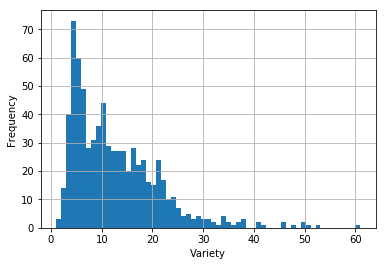
\includegraphics[height=5cm]{fig1}
\caption{Variety distribution }
\label{fig1}
\end{center}
\end{figure}

Projects with more than 10 blocks represent 48.2\% (352 of 730) of the blocks and the scores can be characterized as seen in the following table versus the scores of the projects with less than 10 blocks:

\begin{table}[ht]
\begin{center}
\caption{Comparative table of scores between small and large projects}

\bigskip

\begin{tabular}{|l|l|r|}
\hline
& Large projects & Small projects \\ \hline
Frequency & 352 & 378\\ \hline
Percentage & 48.2 & 51.8\\ \hline
Mean & 18.56 & 9.89\\ \hline
Std. Deviation & 5.33 & 3.27\\ \hline
Minimum & 7 & 3\\ \hline
Maximum & 36 & 19\\ \hline
\end{tabular}
\end{center}
\end{table}



\paragraph{Fourth Level Heading}

Fourth level headings must be flush left, initial caps and roman type.
One line space before the fourth level heading and $1/2$ line
space after the fourth level heading.

\subsection{Citations In Text}

Citations within the text should indicate the author's last name and
year\cite{Knuth-vol3}. Reference style\cite{Comer-btree}
should follow the style that you are used to using, as long as the
citation style is consistent.

\subsubsection{Footnotes}

Indicate footnotes with a number\footnote{This is a sample footnote} in
the text. Place the footnotes at the bottom of the page they appear on.
Precede the footnote with a vertical rule of 2 inches (12 picas).

\subsubsection{Figures}

All artwork must be centered, neat, clean and legible. Do not use pencil
or hand-drawn artwork. Figure number and caption always appear after the
the figure. Place one line space before the figure, one line space
before the figure caption and one line space after the figure caption.
The figure caption is initial caps and each figure is numbered
consecutively.

Make sure that the figure caption does not get separated from the
figure. Leave extra white space at the bottom of the page to avoid
splitting the figure and figure caption.

Figure \ref{fig1} shows how to include a figure as encapsulated postscript.
The source of the figure is in file {\tt fig1.eps}.

Below is another figure using LaTeX commands.


\begin{figure}[ht]
\begin{center}
\setlength{\unitlength}{1pt}
\footnotesize
\begin{picture}(160,80)
        \put(0,0){\framebox(160,80)[]{}}
        \put(10,35){\framebox(80,40){}}
        \put(100,20){\framebox(40,20){}}
        \put(70,10){\framebox(20,10){}}
        \put(20,5){\framebox(10,5){}}
\end{picture}
\caption{Sample Figure Caption}
\end{center}
\end{figure}

\subsubsection{Tables}

All tables must be centered, neat, clean and legible. Do not use pencil
or hand-drawn tables. Table number and title always appear before the
table.

One line space before the table title, one line space after the table
title and one line space after the table. The table title must be
initial caps and each table numbered consecutively.

\begin{table}[ht]
\begin{center}
\caption{Sample Table}

\bigskip

\begin{tabular}{|l|l|r|}
\hline
A & B & 1\\ \hline
C & D & 2\\
E & F & 3\\ \hline
\end{tabular}
\end{center}
\end{table}


\subsubsection{Handling References}

Use a first level heading for the references. References follow the
acknowledgements.


\subsubsection{Acknowledgements}

Use a third level heading for the acknowledgements. All acknowledgements
go at the end of the paper.




%\bibliographystyle{alpha} 
%\bibliography{samplebib}
%inline the .bbl file directly for mailing to authors.

\begin{thebibliography}{Com79}

\bibitem[Com79]{Comer-btree}
D.~Comer.
\newblock The ubiquitous b-tree.
\newblock {\em Computing Surveys}, 11(2):121--137, June 1979.

\bibitem[Knu73]{Knuth-vol3}
D.~E. Knuth.
\newblock {\em The Art of Computer Programming -- Volume 3 / Sorting and
  Searching}.
\newblock Addison-Wesley, 1973.

\end{thebibliography}

\end{document}


